\subsubsection{Functional Principle} \label{subsection:license-google-functional}
%START TEXT INPUT
This is my real text! Rest might be copied or not be checked!
%START TEXT INPUT

%
integrate into application by developer, allows simple checking and callback process with google
asks google play app whether the app was bought on the appstore by the user, takes care of the complicated process (webservice, network etc)
on respond google app passes response to the callback
\begin{figure}[h]
    \centering
    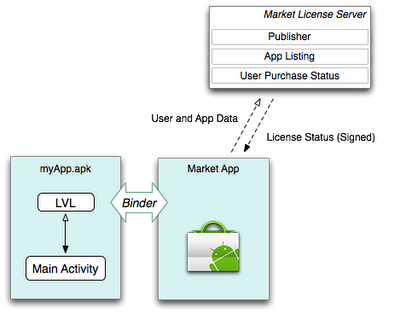
\includegraphics[width=0.8\textwidth]{data/lvl.png}
    \caption{lvl \cite{developersLicensingBlog}}
    \label{fig:lvl}
\end{figure}

determine license status of an app, licensing service needs two informaiton:
- package name of app, a nunce that has to be present in every server response to esnure attacker security, callback for async handling of server respone, implemented in initial license check - user
- specific info user and device such as primary google acc and imsi, collected and provided by google play - google play

security of response important
every published app in playstore, play generates public/private key pair, developer gets public key
public key is embedded into app
google play licensing server signes response with app private key
public key used to check signature of response, effective mechanism is established to ensure origin and detect tampering
\cite{munteanLicense}
%

The information about the application, the device and the user goes off to Google's servers.
Google then checks your name against the list of people it knows have paid for the application on Google Play. (It could also check the name of the application against a list of applications it knows that you've downloaded from Google Play)
If it can see that you have downloaded (and paid for) the application from Google Play it sends back that you have a license, if not then it tells the app you don't.

%
request starts when app initiates to service on Google Play client application
Google Play sends request to licensign server and receives result
google play passes it to app and app decides what happens
\cite{developersLicensingOverview}
%


%
network based service lets query trusted Google Play licensign server, determine whether application is licensed for current user based on buyers database
when, and how often, you want your application to check its license
control over how it handles the response, verifies the signed response data, and enforces access controls

need internet, Google account (else you werent able to buy the applciations), google play installed
addng licensing to app does not affect way the app functions when run on a device that does not offer GOogle Play

replace as copy protection
flexible, secure mechanism for controlling access to applciation
replaces copy protection mechanism which is no longer supported that was previously offered on Google play
license based model that is enforceable on all devices that have acces to google play
access is not bound to characteristics of host device, but google play and licensing policy definded
can be installed, manages on any device and any storage, even SD card
\cite{developersLicensingOverview}
%
